% !TEX root = migratedoc.tex
\chapter{Data models}

\myabstract{A short overview of the different datatypes and how multiple loci are summarized.}

\migrate\ allows for several different input data types, such as electrophoretic marker data, microsatellite data, sequence data as stretches of contiguous sites and as single nucleotide polymorphisms.
 
\section{Infinite allele model}
This assumes 
that every 
mutation will 
result in a new 
allele, there is no back mutation (Fig. \ref{EPFIG}). This model is used in all current implementations of electrophoretic data analyses packages (Biosys-1, GDA among others)
and perhaps is appropriate for this kind of data. \migrate is calculating the parameters for 
each locus independently and summarizes at the end taking the likelihood surfaces or Posterior distributions of each locus into account.
\begin{figure}[thb]
\begin{center}
\makebox[1in]{

\includegraphics[scale=0.6]{mim/ep_graph}}
\end{center}
\caption{Left: Mobility of electrophoretic marker in an electric field. the alleles a,b,c,.. describe a possible sequence of mutation, their mobility is not correlated with the mutational history. Right: The probability that a given allele is not mutating during some time, 
this is a simple exponential relationship.}
\label{EPFIG}
\end{figure}
%\afterpage{\clearpage}
\newpage
\section{Microsatellite model}
\subsection{Ladder model}
The ladder model was invented by cite{ohta:1973:amm} and \cite{kimura:1978:ste} for electrophoretic markers, but was  not as good as expected in describing real electrophoretic alleles. For microsatellites this model seems
much more appropriate cite[e.g. ][]{valdes:1993:afm}, but see \cite{rienzo:1994:mps}, here obviously change happens mostly by slippage of the two DNA strands
creating with higher probability a new allele which is only 1 step apart from the old than one
which 2 steps apart (Fig. \ref{MSATFIG}). 
\begin{figure}[thb]
\begin{center}
\makebox[1in]{

\includegraphics[scale=0.6]{mim/msat_graph}}
\end{center}
\caption{Left: Number of repeat changes of a microsatellite marker. The probability to have a slippage of only one repeat is higher than the slippage of more than one repeat, in a given time, here time=0.1. Right: The probability that a change of 0,1,2,.. steps is occurring during some time.}
\label{MSATFIG}
\end{figure}
%\afterpage{\clearpage}

\subsection{Brownian motion approximation to the ladder model}
This replaces the discrete stepwise mutation model with a continuous Brownian motion model
The results are very similar to the exact stepwise mutation model, but the parameter
estimation is several times faster. This is a crude approximation that has some difficulties when the dataset is not very variable because it uses a cutoff for the the probability that there is no change between two points on a branch, during a time of x  the Brownian motion approximation replaces discrete jumps between repeats with a continuous approximation.
\begin{figure}[thb]
\begin{center}
\makebox[1in]{
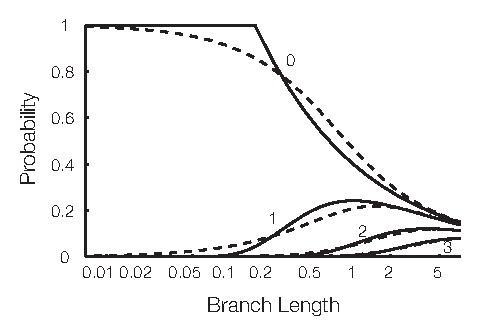
\includegraphics[height=2in]{mim/brownian-stepwise}}
\end{center}
\caption{Comparison of stepwise mutation model with Brownian motion approximation (dashed lines).  The numbers 0, 1, 2, 3, 4 are the number of steps. The Brownian motion approximation for no change is truncated at 1. With steps of more than 4 there is no differences between the stepwise model and the approximation. X-Axis is in log$_10$}
\label{BROWNFIG}
\end{figure}

 
\section{DNA/RNA model}
\subsection{Sequence model}
Migrate implements the sequence model of Felsenstein (1984)  available in {\texttt{dnaml}} (PHYLIP 4.0, Felsenstein 1997)(Fig. \ref{SEQFIG}). The transition probabilities were published by Kishino and Hasegawa (1989).  {\migrate} does not allow for recombination within a locus and therefore may over-estimate variability because of recombination, but this bias is not explored well, if in doubt I suggest to try to run \migrate, simulated high recombination rate data leads to difficulties with convergence. Applications of recombination tests beforehand may work well, but most of these recombination recognition program use the 4-gamete test that is based on the infinite sites model and therefore will overestimate the importance of recombination.\\
Like {\texttt{dnaml}}, {\migrate} also allows for different evolutionary rates, mutation categories and autocorrelation, although
any use of these additional features can slow done to program to a crawl, but this may change
in the future as computers double their speed roughly every 2 years.
\begin{figure}[b]
\begin{center}
\makebox[1in]{

\includegraphics[scale=0.7]{mim/seq_graph}}
\end{center}
\caption{Left: Sequence mutation model. 
Transitions are are shown in black lines, transversion are 
shown with dotted lines.
Right: The probability that a transition or transversion is occurring during some time.
The shown graph uses equal base frequencies, but the used model does not need this restriction.}
\label{SEQFIG}
\end{figure}
%\afterpage{\clearpage}
\subsection{Single nucleotide polymorphism data (SNP)}
We use a rather restrictive ascertainment 
models for SNPs \cite{kuhner:2000:usn}. A better approach than using SNPs is the use of short reads which may or many not contain SNPs. I find that SNPs are an inferior datatype because commonly researchers are adding criteria such as a minor SNP allele must occur at a frequency higher than $x$, and singletons are excluded etc. 
%Currently there are two versions implemented. 
%If you want to use the SNP options, please contact me before
%you run large scale analyses. 
\begin{enumerate}
\item We have
found ALL variable sites and use them even if there are only a few
members of another alleles present. In principal it is as you would
sequence a stretch of DNA and then remove the invariant sites.
Each stretch is treated as completely linked. You can combine many of 
such ``loci'' to improve your estimates.
%\item SNP were developed from a panel population of which we know the
%number of individuals, and that the markers developed were variable, but
%we do not know the actual nucleotides for the individuals [Not fully tested].
\end{enumerate}
This is certainly not how people develop SNPs, but currently the closest
we can come up with.
The SNP coding is otherwise exactly the same as the coding for DNA data.
\par
%If you want to assume that each SNP is unlinked then you need to 
%code each SNP like a sequence data locus with one nucleotide
%(see the examples for sequences),
%I have run successfully 50 SNP loci on a laptop using 40 MB of RAM.
%But there may be better ways to run loci consisting of only one site.

\section{Combining multiple loci}
\migrate calculates all loci estimates independently, the multi-locus estimate is not a simple average over all loci, but takes into account the likelihood or posterior distribution for each parameter at each locus. Loci with flat likelihood curves or flat posteriors will not contribute as much as those with strongly peaked distributions. \migrate offers different treatment in the mutation menu of the parameter menu for the mutation rate among loci:
\begin{center}
\begin{minipage}[c]{12cm}
\begin{verbatim}
Mutation rate among loci
(C)onstant    All loci have the same mutation rate [default]
(E)stimate    Mutation rate 
(V)arying     Mutation rates are different among loci [user input]
(R)elative    Mutation rates estimated from data
\end{verbatim}
\end{minipage}
\end{center}
The {\textbf{Constant}} assumption forces each locus to have the same identical mutation rate. Try this first, because it is the least complicated and most often gives fine results. The {\textbf{Estimate}} is the most difficult and needs dated samples, without sample dates do not use this option.
%one and may often fail, because your data does not contain many loci, or the run has some some loci that did not converge well. With Maximum likelihood this option tries to fit a gamma distribution with a parameter alpha assuming that there is a mean mutation rate for all loci with a rate modifier with shape parameter $\alpha>0$ and $\beta = 1.0$. This results in allowing for variation among loci due to mutation. This often is very difficult to run to convergence. Bayesian inference tries to estimate the rate modifier for each locus, but this seems to work only when information about the dates of the samples is present, and even then it may fail [this needs more work]. 
The last two options, {\textbf{Varying and Relative}}, are probably the best ones to try if you really need variable mutation rates. When you know the relative differences of mutation rates in your data, you can specify them. Alternatively, let \migrate estimate the relative mutation rate using your data. For sequences \migrate calculates a simple Watterson's effective population size estimate over all samples and for each locus and then uses that to calculate a relative mutation rate. With microsatellites and allozyme data \migrate counts the number of alleles and uses those as a measure of relative mutation rates. The mean of these rates is 1.0.
\newpage
